% Created by tikzDevice version 0.12.3.2 on 2022-02-09 23:00:23
% !TEX encoding = UTF-8 Unicode
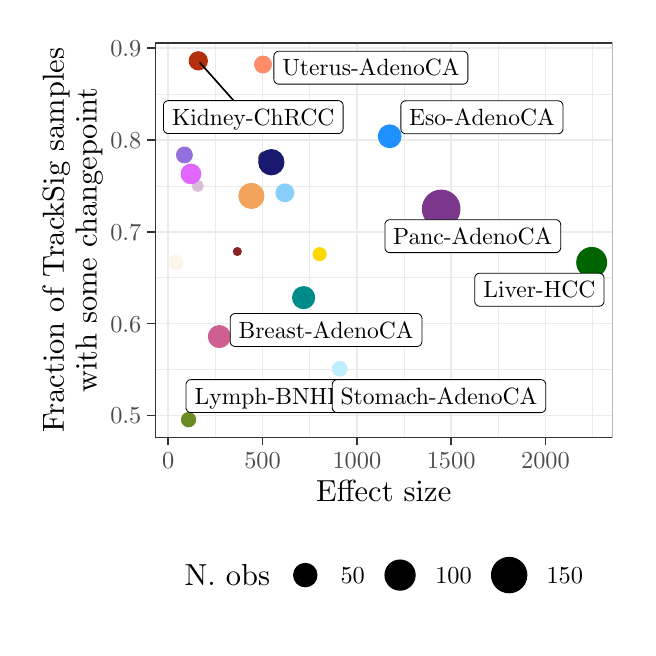
\begin{tikzpicture}[x=1pt,y=1pt]
\definecolor{fillColor}{RGB}{255,255,255}
\path[use as bounding box,fill=fillColor,fill opacity=0.00] (0,0) rectangle (216.81,216.81);
\begin{scope}
\path[clip] (  0.00,  0.00) rectangle (216.81,216.81);
\definecolor{drawColor}{RGB}{255,255,255}
\definecolor{fillColor}{RGB}{255,255,255}

\path[draw=drawColor,line width= 0.6pt,line join=round,line cap=round,fill=fillColor] (  0.00,  0.00) rectangle (216.81,216.81);
\end{scope}
\begin{scope}
\path[clip] ( 46.04, 68.68) rectangle (211.31,211.31);
\definecolor{fillColor}{RGB}{255,255,255}

\path[fill=fillColor] ( 46.04, 68.68) rectangle (211.31,211.31);
\definecolor{drawColor}{gray}{0.92}

\path[draw=drawColor,line width= 0.3pt,line join=round] ( 46.04, 93.29) --
	(211.31, 93.29);

\path[draw=drawColor,line width= 0.3pt,line join=round] ( 46.04,126.45) --
	(211.31,126.45);

\path[draw=drawColor,line width= 0.3pt,line join=round] ( 46.04,159.61) --
	(211.31,159.61);

\path[draw=drawColor,line width= 0.3pt,line join=round] ( 46.04,192.77) --
	(211.31,192.77);

\path[draw=drawColor,line width= 0.3pt,line join=round] ( 67.83, 68.68) --
	( 67.83,211.31);

\path[draw=drawColor,line width= 0.3pt,line join=round] (101.91, 68.68) --
	(101.91,211.31);

\path[draw=drawColor,line width= 0.3pt,line join=round] (135.99, 68.68) --
	(135.99,211.31);

\path[draw=drawColor,line width= 0.3pt,line join=round] (170.06, 68.68) --
	(170.06,211.31);

\path[draw=drawColor,line width= 0.3pt,line join=round] (204.14, 68.68) --
	(204.14,211.31);

\path[draw=drawColor,line width= 0.6pt,line join=round] ( 46.04, 76.71) --
	(211.31, 76.71);

\path[draw=drawColor,line width= 0.6pt,line join=round] ( 46.04,109.87) --
	(211.31,109.87);

\path[draw=drawColor,line width= 0.6pt,line join=round] ( 46.04,143.03) --
	(211.31,143.03);

\path[draw=drawColor,line width= 0.6pt,line join=round] ( 46.04,176.19) --
	(211.31,176.19);

\path[draw=drawColor,line width= 0.6pt,line join=round] ( 46.04,209.35) --
	(211.31,209.35);

\path[draw=drawColor,line width= 0.6pt,line join=round] ( 50.80, 68.68) --
	( 50.80,211.31);

\path[draw=drawColor,line width= 0.6pt,line join=round] ( 84.87, 68.68) --
	( 84.87,211.31);

\path[draw=drawColor,line width= 0.6pt,line join=round] (118.95, 68.68) --
	(118.95,211.31);

\path[draw=drawColor,line width= 0.6pt,line join=round] (153.02, 68.68) --
	(153.02,211.31);

\path[draw=drawColor,line width= 0.6pt,line join=round] (187.10, 68.68) --
	(187.10,211.31);
\definecolor{drawColor}{RGB}{255,215,0}
\definecolor{fillColor}{RGB}{255,215,0}

\path[draw=drawColor,line width= 0.4pt,line join=round,line cap=round,fill=fillColor] (105.51,134.96) circle (  2.34);
\definecolor{drawColor}{RGB}{205,96,144}
\definecolor{fillColor}{RGB}{205,96,144}

\path[draw=drawColor,line width= 0.4pt,line join=round,line cap=round,fill=fillColor] ( 69.26,105.18) circle (  3.96);
\definecolor{drawColor}{gray}{0.24}
\definecolor{fillColor}{gray}{0.24}

\path[draw=drawColor,line width= 0.4pt,line join=round,line cap=round,fill=fillColor] ( 85.78,169.72) circle (  2.26);
\definecolor{drawColor}{RGB}{216,191,216}
\definecolor{fillColor}{RGB}{216,191,216}

\path[draw=drawColor,line width= 0.4pt,line join=round,line cap=round,fill=fillColor] ( 61.46,159.61) circle (  1.99);
\definecolor{drawColor}{RGB}{25,25,112}
\definecolor{fillColor}{RGB}{25,25,112}

\path[draw=drawColor,line width= 0.4pt,line join=round,line cap=round,fill=fillColor] ( 88.05,168.19) circle (  4.55);
\definecolor{drawColor}{RGB}{30,144,255}
\definecolor{fillColor}{RGB}{30,144,255}

\path[draw=drawColor,line width= 0.4pt,line join=round,line cap=round,fill=fillColor] (130.81,177.56) circle (  4.09);
\definecolor{drawColor}{RGB}{139,35,35}
\definecolor{fillColor}{RGB}{139,35,35}

\path[draw=drawColor,line width= 0.4pt,line join=round,line cap=round,fill=fillColor] ( 75.76,135.92) circle (  1.43);
\definecolor{drawColor}{RGB}{179,47,11}
\definecolor{fillColor}{RGB}{179,47,11}

\path[draw=drawColor,line width= 0.4pt,line join=round,line cap=round,fill=fillColor] ( 61.66,204.83) circle (  3.28);
\definecolor{drawColor}{RGB}{0,100,0}
\definecolor{fillColor}{RGB}{0,100,0}

\path[draw=drawColor,line width= 0.4pt,line join=round,line cap=round,fill=fillColor] (203.80,131.98) circle (  5.39);
\definecolor{drawColor}{RGB}{253,245,230}
\definecolor{fillColor}{RGB}{253,245,230}

\path[draw=drawColor,line width= 0.4pt,line join=round,line cap=round,fill=fillColor] ( 53.55,131.98) circle (  2.54);
\definecolor{drawColor}{RGB}{105,139,34}
\definecolor{fillColor}{RGB}{105,139,34}

\path[draw=drawColor,line width= 0.4pt,line join=round,line cap=round,fill=fillColor] ( 58.14, 75.16) circle (  2.56);
\definecolor{drawColor}{RGB}{244,163,93}
\definecolor{fillColor}{RGB}{244,163,93}

\path[draw=drawColor,line width= 0.4pt,line join=round,line cap=round,fill=fillColor] ( 80.84,156.01) circle (  4.53);
\definecolor{drawColor}{RGB}{0,139,139}
\definecolor{fillColor}{RGB}{0,139,139}

\path[draw=drawColor,line width= 0.4pt,line join=round,line cap=round,fill=fillColor] ( 99.71,119.26) circle (  3.98);
\definecolor{drawColor}{RGB}{122,55,139}
\definecolor{fillColor}{RGB}{122,55,139}

\path[draw=drawColor,line width= 0.4pt,line join=round,line cap=round,fill=fillColor] (149.42,151.32) circle (  6.78);
\definecolor{drawColor}{RGB}{224,102,255}
\definecolor{fillColor}{RGB}{224,102,255}

\path[draw=drawColor,line width= 0.4pt,line join=round,line cap=round,fill=fillColor] ( 58.99,163.97) circle (  3.54);
\definecolor{drawColor}{RGB}{135,206,250}
\definecolor{fillColor}{RGB}{135,206,250}

\path[draw=drawColor,line width= 0.4pt,line join=round,line cap=round,fill=fillColor] ( 92.93,157.13) circle (  3.20);
\definecolor{drawColor}{RGB}{191,239,255}
\definecolor{fillColor}{RGB}{191,239,255}

\path[draw=drawColor,line width= 0.4pt,line join=round,line cap=round,fill=fillColor] (112.76, 93.53) circle (  2.64);
\definecolor{drawColor}{RGB}{147,112,219}
\definecolor{fillColor}{RGB}{147,112,219}

\path[draw=drawColor,line width= 0.4pt,line join=round,line cap=round,fill=fillColor] ( 56.64,170.81) circle (  2.84);
\definecolor{drawColor}{RGB}{255,140,105}
\definecolor{fillColor}{RGB}{255,140,105}

\path[draw=drawColor,line width= 0.4pt,line join=round,line cap=round,fill=fillColor] ( 85.04,203.50) circle (  3.04);
\end{scope}
\begin{scope}
\path[clip] ( 46.04, 68.68) rectangle (211.31,211.31);
\definecolor{drawColor}{RGB}{0,0,0}

\path[draw=drawColor,line width= 0.6pt,line join=round,line cap=round] ( 74.43,190.44) -- ( 62.29,204.12);
\definecolor{fillColor}{RGB}{255,255,255}

\path[draw=drawColor,line width= 0.3pt,line join=round,line cap=round,fill=fillColor] ( 75.01,101.61) --
	(140.66,101.61) --
	(140.59,101.62) --
	(140.88,101.63) --
	(141.16,101.69) --
	(141.44,101.79) --
	(141.69,101.93) --
	(141.91,102.12) --
	(142.11,102.34) --
	(142.26,102.58) --
	(142.37,102.85) --
	(142.44,103.13) --
	(142.47,103.42) --
	(142.47,103.42) --
	(142.47,111.71) --
	(142.47,111.71) --
	(142.44,112.00) --
	(142.37,112.28) --
	(142.26,112.55) --
	(142.11,112.79) --
	(141.91,113.01) --
	(141.69,113.20) --
	(141.44,113.34) --
	(141.16,113.44) --
	(140.88,113.50) --
	(140.66,113.52) --
	( 75.01,113.52) --
	( 75.22,113.50) --
	( 74.93,113.51) --
	( 74.64,113.48) --
	( 74.36,113.40) --
	( 74.10,113.27) --
	( 73.86,113.11) --
	( 73.65,112.91) --
	( 73.48,112.67) --
	( 73.34,112.42) --
	( 73.25,112.14) --
	( 73.20,111.85) --
	( 73.20,111.71) --
	( 73.20,103.42) --
	( 73.20,103.57) --
	( 73.20,103.28) --
	( 73.25,102.99) --
	( 73.34,102.71) --
	( 73.48,102.46) --
	( 73.65,102.22) --
	( 73.86,102.02) --
	( 74.10,101.86) --
	( 74.36,101.73) --
	( 74.64,101.65) --
	( 74.93,101.62) --
	cycle;
\end{scope}
\begin{scope}
\path[clip] ( 46.04, 68.68) rectangle (211.31,211.31);
\definecolor{drawColor}{RGB}{0,0,0}

\node[text=drawColor,anchor=base,inner sep=0pt, outer sep=0pt, scale=  0.85] at (107.83,104.63) {Breast-AdenoCA};
\definecolor{fillColor}{RGB}{255,255,255}

\path[draw=drawColor,line width= 0.3pt,line join=round,line cap=round,fill=fillColor] (136.65,178.47) --
	(191.62,178.47) --
	(191.54,178.48) --
	(191.83,178.49) --
	(192.12,178.55) --
	(192.39,178.65) --
	(192.64,178.79) --
	(192.87,178.98) --
	(193.06,179.20) --
	(193.21,179.44) --
	(193.33,179.71) --
	(193.40,179.99) --
	(193.42,180.28) --
	(193.42,180.28) --
	(193.42,188.57) --
	(193.42,188.57) --
	(193.40,188.86) --
	(193.33,189.14) --
	(193.21,189.41) --
	(193.06,189.65) --
	(192.87,189.87) --
	(192.64,190.06) --
	(192.39,190.20) --
	(192.12,190.30) --
	(191.83,190.36) --
	(191.62,190.38) --
	(136.65,190.38) --
	(136.87,190.36) --
	(136.58,190.37) --
	(136.29,190.34) --
	(136.01,190.26) --
	(135.75,190.13) --
	(135.51,189.97) --
	(135.30,189.77) --
	(135.12,189.53) --
	(134.99,189.28) --
	(134.90,189.00) --
	(134.85,188.71) --
	(134.84,188.57) --
	(134.84,180.28) --
	(134.85,180.43) --
	(134.85,180.14) --
	(134.90,179.85) --
	(134.99,179.57) --
	(135.12,179.31) --
	(135.30,179.08) --
	(135.51,178.88) --
	(135.75,178.72) --
	(136.01,178.59) --
	(136.29,178.51) --
	(136.58,178.48) --
	cycle;
\end{scope}
\begin{scope}
\path[clip] ( 46.04, 68.68) rectangle (211.31,211.31);
\definecolor{drawColor}{RGB}{0,0,0}

\node[text=drawColor,anchor=base,inner sep=0pt, outer sep=0pt, scale=  0.85] at (164.13,181.48) {Eso-AdenoCA};
\definecolor{fillColor}{RGB}{255,255,255}

\path[draw=drawColor,line width= 0.3pt,line join=round,line cap=round,fill=fillColor] ( 50.85,178.54) --
	(112.17,178.54) --
	(112.10,178.54) --
	(112.39,178.55) --
	(112.67,178.61) --
	(112.95,178.71) --
	(113.20,178.86) --
	(113.42,179.04) --
	(113.62,179.26) --
	(113.77,179.50) --
	(113.89,179.77) --
	(113.95,180.05) --
	(113.98,180.34) --
	(113.98,180.34) --
	(113.98,188.63) --
	(113.98,188.63) --
	(113.95,188.92) --
	(113.89,189.20) --
	(113.77,189.47) --
	(113.62,189.72) --
	(113.42,189.93) --
	(113.20,190.12) --
	(112.95,190.26) --
	(112.67,190.37) --
	(112.39,190.42) --
	(112.17,190.44) --
	( 50.85,190.44) --
	( 51.07,190.42) --
	( 50.78,190.44) --
	( 50.49,190.40) --
	( 50.21,190.32) --
	( 49.95,190.19) --
	( 49.71,190.03) --
	( 49.50,189.83) --
	( 49.33,189.60) --
	( 49.19,189.34) --
	( 49.10,189.06) --
	( 49.05,188.78) --
	( 49.05,188.63) --
	( 49.05,180.34) --
	( 49.05,180.49) --
	( 49.05,180.20) --
	( 49.10,179.91) --
	( 49.19,179.63) --
	( 49.33,179.38) --
	( 49.50,179.14) --
	( 49.71,178.94) --
	( 49.95,178.78) --
	( 50.21,178.65) --
	( 50.49,178.57) --
	( 50.78,178.54) --
	cycle;
\end{scope}
\begin{scope}
\path[clip] ( 46.04, 68.68) rectangle (211.31,211.31);
\definecolor{drawColor}{RGB}{0,0,0}

\node[text=drawColor,anchor=base,inner sep=0pt, outer sep=0pt, scale=  0.85] at ( 81.51,181.55) {Kidney-ChRCC};
\definecolor{fillColor}{RGB}{255,255,255}

\path[draw=drawColor,line width= 0.3pt,line join=round,line cap=round,fill=fillColor] (163.37,116.17) --
	(206.46,116.17) --
	(206.38,116.17) --
	(206.67,116.18) --
	(206.96,116.24) --
	(207.23,116.34) --
	(207.48,116.49) --
	(207.71,116.67) --
	(207.90,116.89) --
	(208.06,117.13) --
	(208.17,117.40) --
	(208.24,117.68) --
	(208.26,117.97) --
	(208.26,117.97) --
	(208.26,126.26) --
	(208.26,126.26) --
	(208.24,126.55) --
	(208.17,126.83) --
	(208.06,127.10) --
	(207.90,127.35) --
	(207.71,127.57) --
	(207.48,127.75) --
	(207.23,127.89) --
	(206.96,128.00) --
	(206.67,128.06) --
	(206.46,128.07) --
	(163.37,128.07) --
	(163.59,128.06) --
	(163.30,128.07) --
	(163.01,128.03) --
	(162.73,127.95) --
	(162.47,127.83) --
	(162.23,127.66) --
	(162.02,127.46) --
	(161.84,127.23) --
	(161.71,126.97) --
	(161.61,126.69) --
	(161.57,126.41) --
	(161.56,126.26) --
	(161.56,117.97) --
	(161.57,118.12) --
	(161.57,117.83) --
	(161.61,117.54) --
	(161.71,117.27) --
	(161.84,117.01) --
	(162.02,116.78) --
	(162.23,116.57) --
	(162.47,116.41) --
	(162.73,116.28) --
	(163.01,116.20) --
	(163.30,116.17) --
	cycle;
\end{scope}
\begin{scope}
\path[clip] ( 46.04, 68.68) rectangle (211.31,211.31);
\definecolor{drawColor}{RGB}{0,0,0}

\node[text=drawColor,anchor=base,inner sep=0pt, outer sep=0pt, scale=  0.85] at (184.91,119.18) {Liver-HCC};
\definecolor{fillColor}{RGB}{255,255,255}

\path[draw=drawColor,line width= 0.3pt,line join=round,line cap=round,fill=fillColor] ( 59.02, 77.73) --
	(114.89, 77.73) --
	(114.82, 77.73) --
	(115.11, 77.74) --
	(115.39, 77.80) --
	(115.66, 77.90) --
	(115.92, 78.05) --
	(116.14, 78.23) --
	(116.33, 78.45) --
	(116.49, 78.69) --
	(116.60, 78.96) --
	(116.67, 79.24) --
	(116.70, 79.53) --
	(116.70, 79.53) --
	(116.70, 87.82) --
	(116.70, 87.82) --
	(116.67, 88.11) --
	(116.60, 88.39) --
	(116.49, 88.66) --
	(116.33, 88.91) --
	(116.14, 89.12) --
	(115.92, 89.31) --
	(115.66, 89.45) --
	(115.39, 89.56) --
	(115.11, 89.61) --
	(114.89, 89.63) --
	( 59.02, 89.63) --
	( 59.24, 89.61) --
	( 58.95, 89.63) --
	( 58.66, 89.59) --
	( 58.38, 89.51) --
	( 58.12, 89.38) --
	( 57.88, 89.22) --
	( 57.67, 89.02) --
	( 57.50, 88.79) --
	( 57.36, 88.53) --
	( 57.27, 88.25) --
	( 57.22, 87.97) --
	( 57.22, 87.82) --
	( 57.22, 79.53) --
	( 57.22, 79.68) --
	( 57.22, 79.39) --
	( 57.27, 79.10) --
	( 57.36, 78.82) --
	( 57.50, 78.57) --
	( 57.67, 78.33) --
	( 57.88, 78.13) --
	( 58.12, 77.97) --
	( 58.38, 77.84) --
	( 58.66, 77.76) --
	( 58.95, 77.73) --
	cycle;
\end{scope}
\begin{scope}
\path[clip] ( 46.04, 68.68) rectangle (211.31,211.31);
\definecolor{drawColor}{RGB}{0,0,0}

\node[text=drawColor,anchor=base,inner sep=0pt, outer sep=0pt, scale=  0.85] at ( 86.96, 80.74) {Lymph-BNHL};
\definecolor{fillColor}{RGB}{255,255,255}

\path[draw=drawColor,line width= 0.3pt,line join=round,line cap=round,fill=fillColor] (130.89,135.51) --
	(190.79,135.51) --
	(190.72,135.51) --
	(191.01,135.52) --
	(191.29,135.58) --
	(191.56,135.69) --
	(191.81,135.83) --
	(192.04,136.01) --
	(192.23,136.23) --
	(192.39,136.48) --
	(192.50,136.75) --
	(192.57,137.03) --
	(192.60,137.32) --
	(192.60,137.32) --
	(192.60,145.61) --
	(192.60,145.61) --
	(192.57,145.90) --
	(192.50,146.18) --
	(192.39,146.45) --
	(192.23,146.69) --
	(192.04,146.91) --
	(191.81,147.09) --
	(191.56,147.24) --
	(191.29,147.34) --
	(191.01,147.40) --
	(190.79,147.41) --
	(130.89,147.41) --
	(131.11,147.40) --
	(130.82,147.41) --
	(130.53,147.38) --
	(130.25,147.29) --
	(129.99,147.17) --
	(129.75,147.01) --
	(129.54,146.80) --
	(129.37,146.57) --
	(129.23,146.31) --
	(129.14,146.04) --
	(129.09,145.75) --
	(129.09,145.61) --
	(129.09,137.32) --
	(129.09,137.46) --
	(129.09,137.17) --
	(129.14,136.89) --
	(129.23,136.61) --
	(129.37,136.35) --
	(129.54,136.12) --
	(129.75,135.92) --
	(129.99,135.75) --
	(130.25,135.63) --
	(130.53,135.55) --
	(130.82,135.51) --
	cycle;
\end{scope}
\begin{scope}
\path[clip] ( 46.04, 68.68) rectangle (211.31,211.31);
\definecolor{drawColor}{RGB}{0,0,0}

\node[text=drawColor,anchor=base,inner sep=0pt, outer sep=0pt, scale=  0.85] at (160.84,138.52) {Panc-AdenoCA};
\definecolor{fillColor}{RGB}{255,255,255}

\path[draw=drawColor,line width= 0.3pt,line join=round,line cap=round,fill=fillColor] (111.88, 77.72) --
	(185.40, 77.72) --
	(185.33, 77.72) --
	(185.62, 77.74) --
	(185.91, 77.79) --
	(186.18, 77.90) --
	(186.43, 78.04) --
	(186.66, 78.23) --
	(186.85, 78.44) --
	(187.00, 78.69) --
	(187.12, 78.96) --
	(187.19, 79.24) --
	(187.21, 79.53) --
	(187.21, 79.53) --
	(187.21, 87.82) --
	(187.21, 87.82) --
	(187.19, 88.11) --
	(187.12, 88.39) --
	(187.00, 88.66) --
	(186.85, 88.90) --
	(186.66, 89.12) --
	(186.43, 89.30) --
	(186.18, 89.45) --
	(185.91, 89.55) --
	(185.62, 89.61) --
	(185.40, 89.62) --
	(111.88, 89.62) --
	(112.10, 89.61) --
	(111.81, 89.62) --
	(111.52, 89.59) --
	(111.24, 89.51) --
	(110.98, 89.38) --
	(110.74, 89.22) --
	(110.53, 89.01) --
	(110.35, 88.78) --
	(110.22, 88.52) --
	(110.12, 88.25) --
	(110.08, 87.96) --
	(110.07, 87.82) --
	(110.07, 79.53) --
	(110.08, 79.67) --
	(110.08, 79.38) --
	(110.12, 79.10) --
	(110.22, 78.82) --
	(110.35, 78.56) --
	(110.53, 78.33) --
	(110.74, 78.13) --
	(110.98, 77.96) --
	(111.24, 77.84) --
	(111.52, 77.76) --
	(111.81, 77.72) --
	cycle;
\end{scope}
\begin{scope}
\path[clip] ( 46.04, 68.68) rectangle (211.31,211.31);
\definecolor{drawColor}{RGB}{0,0,0}

\node[text=drawColor,anchor=base,inner sep=0pt, outer sep=0pt, scale=  0.85] at (148.64, 80.73) {Stomach-AdenoCA};
\definecolor{fillColor}{RGB}{255,255,255}

\path[draw=drawColor,line width= 0.3pt,line join=round,line cap=round,fill=fillColor] ( 90.78,196.40) --
	(157.27,196.40) --
	(157.19,196.40) --
	(157.48,196.41) --
	(157.77,196.47) --
	(158.04,196.57) --
	(158.29,196.72) --
	(158.52,196.90) --
	(158.71,197.12) --
	(158.87,197.36) --
	(158.98,197.63) --
	(159.05,197.91) --
	(159.07,198.20) --
	(159.07,198.20) --
	(159.07,206.49) --
	(159.07,206.49) --
	(159.05,206.78) --
	(158.98,207.06) --
	(158.87,207.33) --
	(158.71,207.58) --
	(158.52,207.80) --
	(158.29,207.98) --
	(158.04,208.12) --
	(157.77,208.23) --
	(157.48,208.29) --
	(157.27,208.30) --
	( 90.78,208.30) --
	( 91.00,208.29) --
	( 90.71,208.30) --
	( 90.42,208.26) --
	( 90.14,208.18) --
	( 89.88,208.06) --
	( 89.64,207.89) --
	( 89.43,207.69) --
	( 89.25,207.46) --
	( 89.12,207.20) --
	( 89.03,206.92) --
	( 88.98,206.64) --
	( 88.97,206.49) --
	( 88.97,198.20) --
	( 88.98,198.35) --
	( 88.98,198.06) --
	( 89.03,197.77) --
	( 89.12,197.50) --
	( 89.25,197.24) --
	( 89.43,197.01) --
	( 89.64,196.80) --
	( 89.88,196.64) --
	( 90.14,196.51) --
	( 90.42,196.43) --
	( 90.71,196.40) --
	cycle;
\end{scope}
\begin{scope}
\path[clip] ( 46.04, 68.68) rectangle (211.31,211.31);
\definecolor{drawColor}{RGB}{0,0,0}

\node[text=drawColor,anchor=base,inner sep=0pt, outer sep=0pt, scale=  0.85] at (124.02,199.41) {Uterus-AdenoCA};
\definecolor{drawColor}{gray}{0.20}

\path[draw=drawColor,line width= 0.6pt,line join=round,line cap=round] ( 46.04, 68.68) rectangle (211.31,211.31);
\end{scope}
\begin{scope}
\path[clip] (  0.00,  0.00) rectangle (216.81,216.81);
\definecolor{drawColor}{gray}{0.30}

\node[text=drawColor,anchor=base east,inner sep=0pt, outer sep=0pt, scale=  0.88] at ( 41.09, 73.68) {0.5};

\node[text=drawColor,anchor=base east,inner sep=0pt, outer sep=0pt, scale=  0.88] at ( 41.09,106.84) {0.6};

\node[text=drawColor,anchor=base east,inner sep=0pt, outer sep=0pt, scale=  0.88] at ( 41.09,140.00) {0.7};

\node[text=drawColor,anchor=base east,inner sep=0pt, outer sep=0pt, scale=  0.88] at ( 41.09,173.16) {0.8};

\node[text=drawColor,anchor=base east,inner sep=0pt, outer sep=0pt, scale=  0.88] at ( 41.09,206.32) {0.9};
\end{scope}
\begin{scope}
\path[clip] (  0.00,  0.00) rectangle (216.81,216.81);
\definecolor{drawColor}{gray}{0.20}

\path[draw=drawColor,line width= 0.6pt,line join=round] ( 43.29, 76.71) --
	( 46.04, 76.71);

\path[draw=drawColor,line width= 0.6pt,line join=round] ( 43.29,109.87) --
	( 46.04,109.87);

\path[draw=drawColor,line width= 0.6pt,line join=round] ( 43.29,143.03) --
	( 46.04,143.03);

\path[draw=drawColor,line width= 0.6pt,line join=round] ( 43.29,176.19) --
	( 46.04,176.19);

\path[draw=drawColor,line width= 0.6pt,line join=round] ( 43.29,209.35) --
	( 46.04,209.35);
\end{scope}
\begin{scope}
\path[clip] (  0.00,  0.00) rectangle (216.81,216.81);
\definecolor{drawColor}{gray}{0.20}

\path[draw=drawColor,line width= 0.6pt,line join=round] ( 50.80, 65.93) --
	( 50.80, 68.68);

\path[draw=drawColor,line width= 0.6pt,line join=round] ( 84.87, 65.93) --
	( 84.87, 68.68);

\path[draw=drawColor,line width= 0.6pt,line join=round] (118.95, 65.93) --
	(118.95, 68.68);

\path[draw=drawColor,line width= 0.6pt,line join=round] (153.02, 65.93) --
	(153.02, 68.68);

\path[draw=drawColor,line width= 0.6pt,line join=round] (187.10, 65.93) --
	(187.10, 68.68);
\end{scope}
\begin{scope}
\path[clip] (  0.00,  0.00) rectangle (216.81,216.81);
\definecolor{drawColor}{gray}{0.30}

\node[text=drawColor,anchor=base,inner sep=0pt, outer sep=0pt, scale=  0.88] at ( 50.80, 57.67) {0};

\node[text=drawColor,anchor=base,inner sep=0pt, outer sep=0pt, scale=  0.88] at ( 84.87, 57.67) {500};

\node[text=drawColor,anchor=base,inner sep=0pt, outer sep=0pt, scale=  0.88] at (118.95, 57.67) {1000};

\node[text=drawColor,anchor=base,inner sep=0pt, outer sep=0pt, scale=  0.88] at (153.02, 57.67) {1500};

\node[text=drawColor,anchor=base,inner sep=0pt, outer sep=0pt, scale=  0.88] at (187.10, 57.67) {2000};
\end{scope}
\begin{scope}
\path[clip] (  0.00,  0.00) rectangle (216.81,216.81);
\definecolor{drawColor}{RGB}{0,0,0}

\node[text=drawColor,anchor=base,inner sep=0pt, outer sep=0pt, scale=  1.10] at (128.67, 45.63) {Effect size};
\end{scope}
\begin{scope}
\path[clip] (  0.00,  0.00) rectangle (216.81,216.81);
\definecolor{drawColor}{RGB}{0,0,0}

\node[text=drawColor,rotate= 90.00,anchor=base,inner sep=0pt, outer sep=0pt, scale=  1.10] at ( 13.08,139.99) {Fraction of TrackSig samples};

\node[text=drawColor,rotate= 90.00,anchor=base,inner sep=0pt, outer sep=0pt, scale=  1.10] at ( 24.96,139.99) {with some changepoint};
\end{scope}
\begin{scope}
\path[clip] (  0.00,  0.00) rectangle (216.81,216.81);
\definecolor{fillColor}{RGB}{255,255,255}

\path[fill=fillColor] ( 51.17,  5.50) rectangle (206.18, 32.49);
\end{scope}
\begin{scope}
\path[clip] (  0.00,  0.00) rectangle (216.81,216.81);
\definecolor{drawColor}{RGB}{0,0,0}

\node[text=drawColor,anchor=base west,inner sep=0pt, outer sep=0pt, scale=  1.10] at ( 56.67, 15.21) {N. obs};
\end{scope}
\begin{scope}
\path[clip] (  0.00,  0.00) rectangle (216.81,216.81);
\definecolor{fillColor}{RGB}{255,255,255}

\path[fill=fillColor] ( 93.08, 11.00) rectangle (107.54, 26.99);
\end{scope}
\begin{scope}
\path[clip] (  0.00,  0.00) rectangle (216.81,216.81);
\definecolor{drawColor}{RGB}{0,0,0}
\definecolor{fillColor}{RGB}{0,0,0}

\path[draw=drawColor,line width= 0.4pt,line join=round,line cap=round,fill=fillColor] (100.31, 19.00) circle (  4.22);
\end{scope}
\begin{scope}
\path[clip] (  0.00,  0.00) rectangle (216.81,216.81);
\definecolor{fillColor}{RGB}{255,255,255}

\path[fill=fillColor] (127.34, 11.00) rectangle (141.79, 26.99);
\end{scope}
\begin{scope}
\path[clip] (  0.00,  0.00) rectangle (216.81,216.81);
\definecolor{drawColor}{RGB}{0,0,0}
\definecolor{fillColor}{RGB}{0,0,0}

\path[draw=drawColor,line width= 0.4pt,line join=round,line cap=round,fill=fillColor] (134.56, 19.00) circle (  5.44);
\end{scope}
\begin{scope}
\path[clip] (  0.00,  0.00) rectangle (216.81,216.81);
\definecolor{fillColor}{RGB}{255,255,255}

\path[fill=fillColor] (165.99, 11.00) rectangle (181.98, 26.99);
\end{scope}
\begin{scope}
\path[clip] (  0.00,  0.00) rectangle (216.81,216.81);
\definecolor{drawColor}{RGB}{0,0,0}
\definecolor{fillColor}{RGB}{0,0,0}

\path[draw=drawColor,line width= 0.4pt,line join=round,line cap=round,fill=fillColor] (173.98, 19.00) circle (  6.38);
\end{scope}
\begin{scope}
\path[clip] (  0.00,  0.00) rectangle (216.81,216.81);
\definecolor{drawColor}{RGB}{0,0,0}

\node[text=drawColor,anchor=base west,inner sep=0pt, outer sep=0pt, scale=  0.88] at (113.04, 15.97) {50};
\end{scope}
\begin{scope}
\path[clip] (  0.00,  0.00) rectangle (216.81,216.81);
\definecolor{drawColor}{RGB}{0,0,0}

\node[text=drawColor,anchor=base west,inner sep=0pt, outer sep=0pt, scale=  0.88] at (147.29, 15.97) {100};
\end{scope}
\begin{scope}
\path[clip] (  0.00,  0.00) rectangle (216.81,216.81);
\definecolor{drawColor}{RGB}{0,0,0}

\node[text=drawColor,anchor=base west,inner sep=0pt, outer sep=0pt, scale=  0.88] at (187.48, 15.97) {150};
\end{scope}
\end{tikzpicture}
